% ********** Rozdział 4 **********
\chapter{Prezentacja warstwy użytkowej projektu}
\subsection{Główne Menu Systemu}
Po uruchomieniu aplikacji, użytkownik natychmiast widzi główne menu, które jest punktem wyjścia do wszystkich funkcji systemu. Menu to prezentuje kilka opcji, takich jak:
\begin{itemize}
    \item Zarządzanie ofertami,
    \item Zarządzanie rezerwacjami,
    \item Zarządzanie płatnościami,
    \item Zarządzanie użytkownikami,
    \item Wyjście z aplikacji.
\end{itemize}

\begin{figure}[htbp]
  \centering
  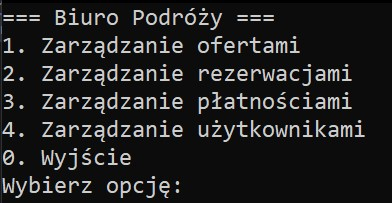
\includegraphics[width=0.8\textwidth]{figures/menu.jpg} 
  \caption{Menu startowe aplikacji}
  \label{fig:obrazek}
\end{figure}

Dzięki tej strukturze, użytkownik może szybko zorientować się w dostępnych funkcjonalnościach oraz łatwo przechodzić do interesującego go modułu.
\newpage
\subsection{Podmenu Modułów}
Każdy z głównych modułów systemu posiada własne podmenu, co pozwala na szczegółową obsługę konkretnej dziedziny:
\begin{itemize}
    \item \textbf{Wyświetlenie wszystkich ofert} – system prezentuje listę ofert, pokazując podstawowe dane, takie jak identyfikator, nazwa, destynacja, cena i liczba dostępnych miejsc.
    \item \textbf{Wyświetlenie szczegółów oferty} – po wprowadzeniu ID konkretnej oferty, system pokazuje wszystkie informacje dotyczące tej oferty.
    \item \textbf{Dodanie nowej oferty} – użytkownik wprowadza dane dotyczące nowej oferty (nazwa, miejsce docelowe, cena, dostępne miejsca), które następnie są zapisywane w systemie.
    \item \textbf{Edycja istniejącej oferty} – umożliwia modyfikację parametrów oferty, na podstawie której system aktualizuje dane w bazie.
    \item \textbf{Usuwanie oferty} – pozwala na usunięcie oferty o podanym ID.
    \item \textbf{Backup ofert} – opcja ta tworzy kopię zapasową pliku zawierającego dane ofert, co zwiększa bezpieczeństwo przechowywanych informacji.
\end{itemize}

\begin{figure}[htbp]
  \centering
  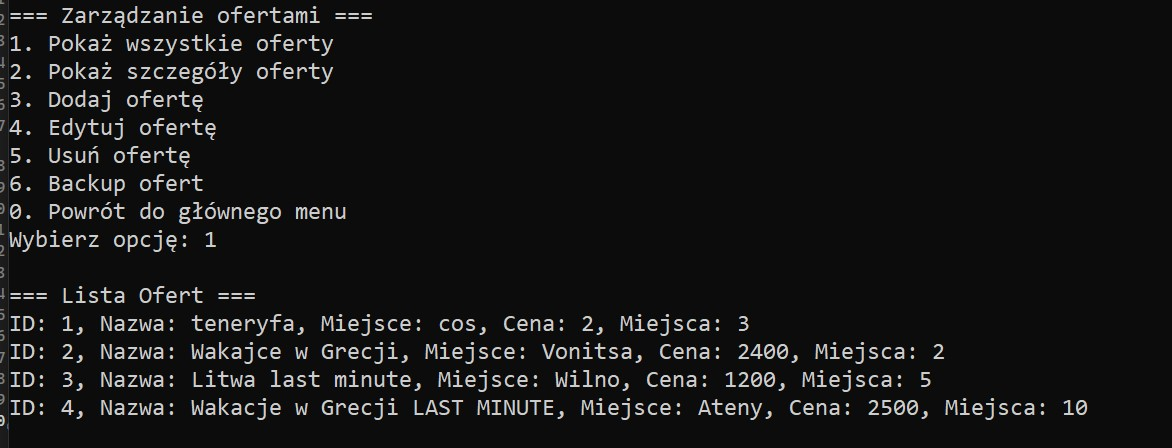
\includegraphics[width=0.9\textwidth]{figures/lista_ofert.jpg} 
  \caption{Zarządzanie ofertami}
  \label{fig:obrazek}
\end{figure}

\subsection{Moduł rezerwacji}
W podmenu rezerwacji użytkownik może:
\begin{itemize}
    \item \textbf{Dodać nową rezerwację} – wprowadzając identyfikator oferty, dane klienta i liczbę miejsc, co pozwala na rejestrację rezerwacji w systemie.
    \item \textbf{Edytować istniejącą rezerwację} – umożliwiając aktualizację danych rezerwacji (np. zmiana liczby miejsc lub korekta danych klienta).
    \item \textbf{Anulować rezerwację} – usuwając rezerwację, gdy zajdzie taka potrzeba.
    \item \textbf{Wyświetlić listę wszystkich rezerwacji} – co pozwala na bieżący przegląd dokonanych rezerwacji.
\end{itemize}
\newpage
\subsection{Moduł rezerwacji - dodawanie rezerwacji}
Poniżej przedstawiony sposób możliwości dodawania rezerwacji: 
\begin{figure}[htbp]
  \centering
  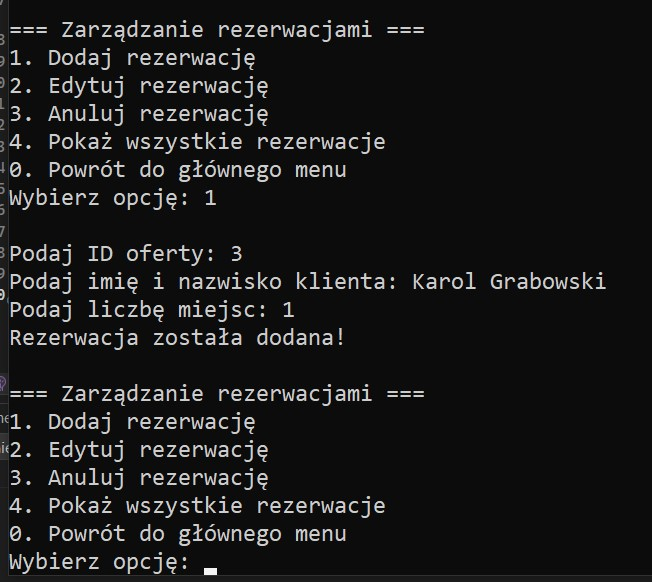
\includegraphics[width=0.9\textwidth]{figures/rezerwacja.jpg} 
  \caption{Zarządzanie rezerwacjami}
  \label{fig:obrazek}
\end{figure}


\subsection{Moduł Płatności}
Podmenu płatności umożliwia:
\begin{itemize}
    \item \textbf{Dodanie nowej płatności} – na podstawie identyfikatora rezerwacji, kwoty i daty płatności.
    \item \textbf{Wyświetlenie listy płatności} – system prezentuje wszystkie dokonane transakcje.
    \item \textbf{Generowanie faktur} – po podaniu ID płatności, system generuje sformatowaną fakturę, zawierającą kluczowe informacje o transakcji.
\end{itemize}


\subsection{Moduł Użytkowników}
\begin{itemize}
    \item \textbf{Dodawanie nowych użytkowników} – umożliwiając rejestrację nowych kont wraz z przypisaniem roli (administrator, pracownik, klient).
    \item \textbf{Edycja danych użytkowników} – co pozwala na aktualizację informacji takich jak nazwa czy przypisana rola.
    \item \textbf{Usuwanie użytkowników} – umożliwiając kontrolę nad dostępem do systemu.
    \item \textbf{Wyświetlanie listy użytkowników} – co pozwala na szybki przegląd dostępnych kont.
\end{itemize}

\section{Interakcja i Walidacja}
Interfejs konsolowy został zaprojektowany tak, aby zapewnić czytelne komunikaty oraz intuicyjne wprowadzanie danych. Każda operacja jest poprzedzona instrukcjami wyświetlanymi na ekranie, a system sprawdza poprawność wprowadzonych danych (np. weryfikacja, czy podana cena ma właściwy format lub czy liczba miejsc jest liczbą całkowitą). Dzięki temu użytkownik otrzymuje natychmiastową informację zwrotną o poprawności swojej operacji, co zmniejsza ryzyko błędów.


\subsection{Zalety Interfejsu Konsolowego}
Mimo że interfejs jest oparty na konsoli, ma on kilka istotnych zalet:
\begin{description}
    \item[Prostota:] System opiera się na przejrzystym menu, co pozwala na szybkie opanowanie obsługi aplikacji nawet przez osoby niezaznajomione z technologiami informatycznymi.
    \item[Łatwość Utrzymania:] Dzięki modularnej budowie menu oraz oddzieleniu logiki biznesowej, przyszłe modyfikacje lub rozbudowa interfejsu są łatwe do wykonania.
    \item[Szybkość Działania:] Aplikacja reaguje natychmiastowo na wprowadzane komendy, co zwiększa efektywność pracy użytkownika.
\end{description}

\section{Podsumowanie warstwy użytkowej}
Warstwa użytkowa systemu "Biuro Podróży" jest kluczowym elementem, który umożliwia użytkownikom efektywną interakcję z systemem. Dzięki dobrze zaprojektowanemu interfejsowi konsolowemu, użytkownicy mogą łatwo przechodzić między różnymi modułami systemu – od zarządzania ofertami, poprzez rezerwacje i płatności, aż po zarządzanie użytkownikami. Jasno zdefiniowane komunikaty oraz mechanizmy walidacji wprowadzanych danych zapewniają stabilność i przejrzystość działania systemu, co stanowi solidną podstawę do dalszej rozbudowy, na przykład o graficzny interfejs użytkownika lub dodatkowe mechanizmy zabezpieczeń.

\section{Poszczególne opcje programu}

\begin{figure}[htbp]
  \centering
  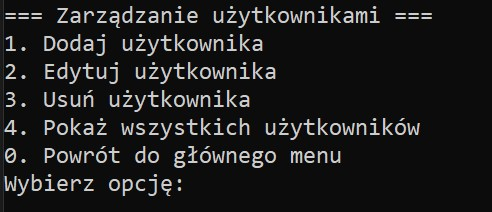
\includegraphics[width=0.9\textwidth]{figures/zarzadzanie_urzytkownikami.jpg} 
  \caption{Zarządzanie użytkownikami}
  \label{fig:obrazek}
\end{figure}

\begin{figure}[htbp]
  \centering
  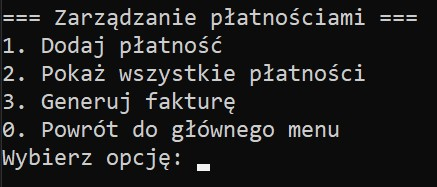
\includegraphics[width=0.9\textwidth]{figures/zarzadzanie_platnosciami.jpg} 
  \caption{Zarządzanie płatnościami}
  \label{fig:obrazek}
\end{figure}


% ********** Koniec rozdziału **********
